\chapter{Ejercicio juego del pañuelo} \label{gripper}
En este capítulo se expone cómo ha sido el desarrollo del juego del pañuelo. Primero hablaremos del enunciado, seguidamente hablaremos de los modelos desarrollados, junto con las herramientas que se han utilizado. Para terminar, se ofrecen dos soluciones de referencia en Python y Scratch.

Para que nuestro ejercicio sea acorde con el juego del pañuelo que conocemos todos y con las competiciones actuales, necesitamos hacer un robot con pinzas, una lata  y un circuito. Las principales tecnologías que se han utilizado en este ejercicio son Blender, JavaScript, A-Frame y Websim .


\section{Enunciado}
El propósito es crear un ejercicio con un nuevo robot que sea capaz de coger objetos y moverlos por el escenario. El nuevo robot debe tener pinzas móviles para atrapar otros objetos. 

El juego del pañuelo es muy popular entre los más pequeños y también en el mundo de la robótica. En las competiciones de robots este juego incluye programar un sigue líneas. El robot debe recorrer un circuito, ser capaz de coger una lata que obstaculiza el camino y volver con ella a la posición de salida. En la Figura 5.1 a y 5.1 b podemos ver cómo es este juego en competiciones de robótica como Robocampeones.

\begin{figure}[H]
  \begin{subfigure}[b]{0.5\textwidth}
  \centering
    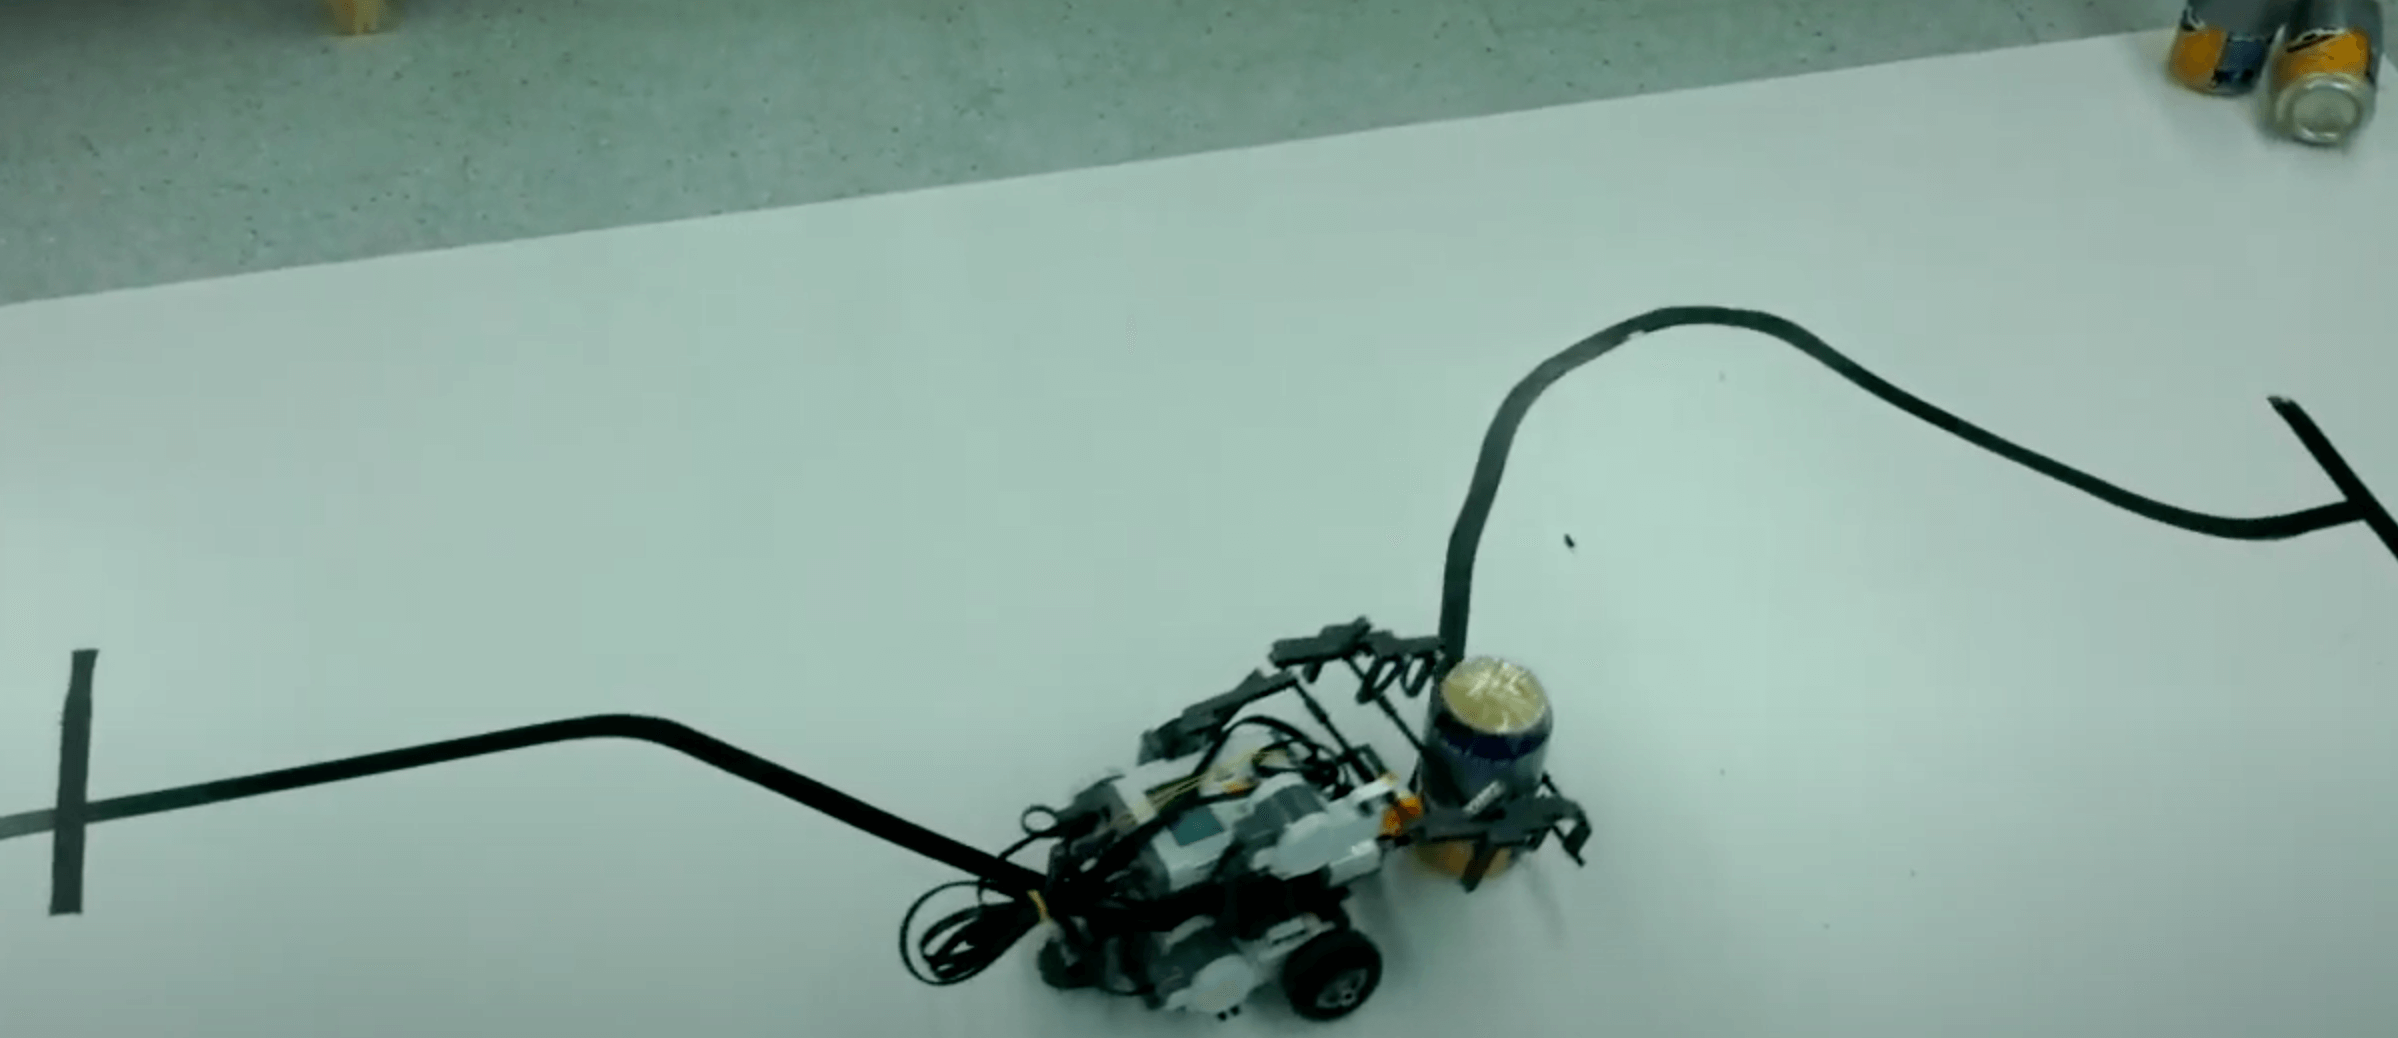
\includegraphics[width=0.95\textwidth, height=0.4\textwidth]{chapters/images/jp.png}
    \caption{Juego del pañuelo con un robot \footnote{https://www.youtube.com/watch?v=FsS2CSudl7c}}
    \label{fig:f1}
  \end{subfigure}
  \hfill
  \begin{subfigure}[b]{0.5\textwidth}
  \centering
    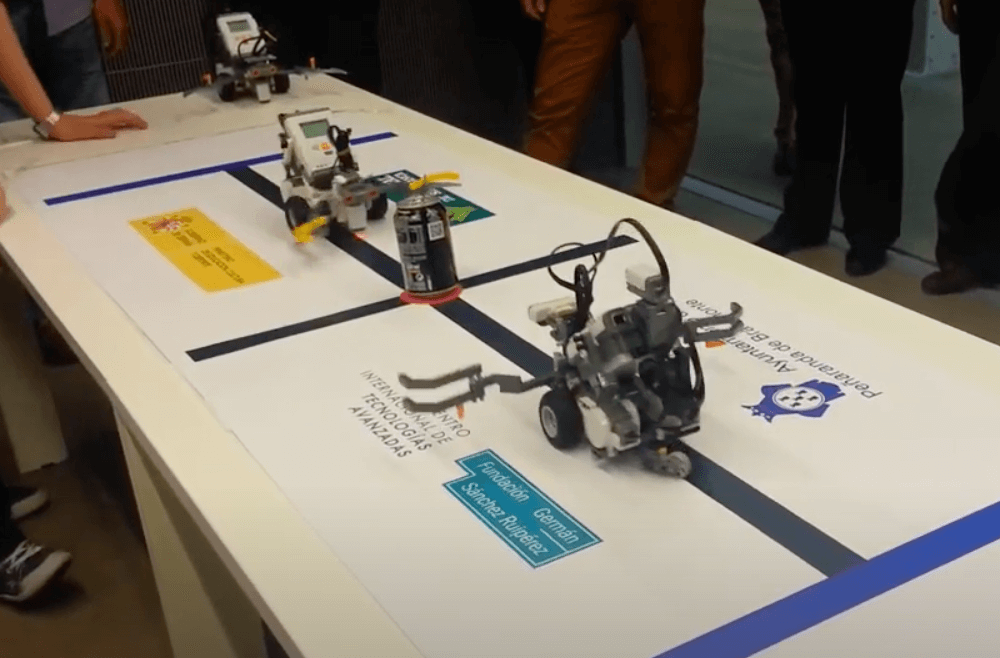
\includegraphics[width=0.95\textwidth, height=0.4\textwidth]{chapters/images/jp2.png}
    \caption{Juego del pañuelo multirobot \footnote{https://www.youtube.com/watch?v=6T\_Ua\-TaB6Q}}
    \label{fig:f2}
  \end{subfigure}
  \caption{Juego del Pañuelo en competiciones robóticas}

\end{figure}

En este trabajo fin de grado hemos hecho nuestra versión del juego del pañuelo basándonos en las competiciones existentes. De esta forma, los alumnos pueden adquirir experiencia y animarse en un futuro a presentarse a competiciones de alto nivel.
 
En este ejercicio el alumno deberá programar en Python o en Scratch, un algoritmo que permita que el Mbot con pinzas avance siguiendo la línea negra del circuito hasta que se encuentre a poca distancia de la lata. Una vez se encuentre enfrente de la lata, el robot debe cerrar las pinzas y dar media vuelta para volver a la casilla de salida, llevando consigo la lata en todo momento. Gracias a un evaluador automático vamos a obtener la puntuación, ésta va a depender del porcentaje de circuito recorrido y si lleva o no la lata entre las pinzas.


Se creó la página web de teoría con HTML5  y se añadió a las plantillas de Django en Kibotics en su versión de Python y Scratch. La teoría relacionada con este ejercicio se muestra en las Figuras 5.2, 5.3, 5.4, 5.5, 5.6 y 5.7. Esta información ayuda a  los alumnos a entender mejor cómo funcionan los sensores y actuadores y sea más sencilla la realización del ejercicio.

\begin{figure}[H]
    \centering
    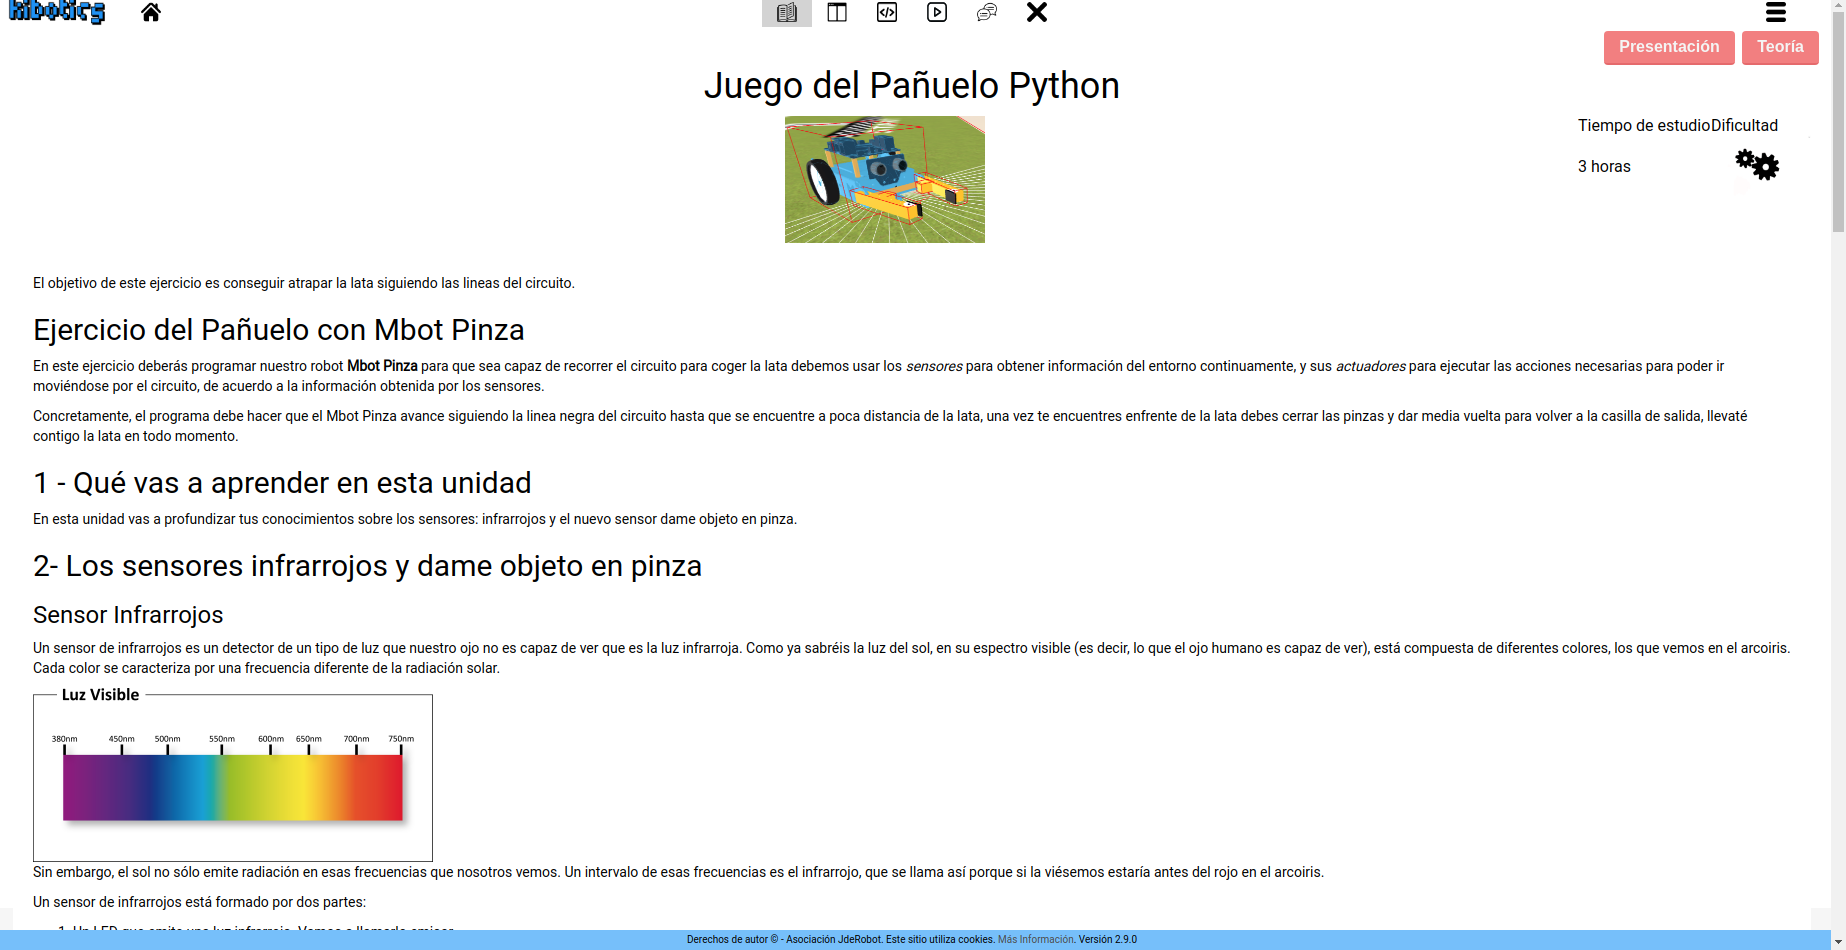
\includegraphics[width=1\textwidth, height=0.45\textwidth]{chapters/images/teoriag1.png}
    \caption{Página de teoría enunciado y requisitos}
    \label{fig:my_label}
\end{figure}
\begin{figure}[H]
    \centering
    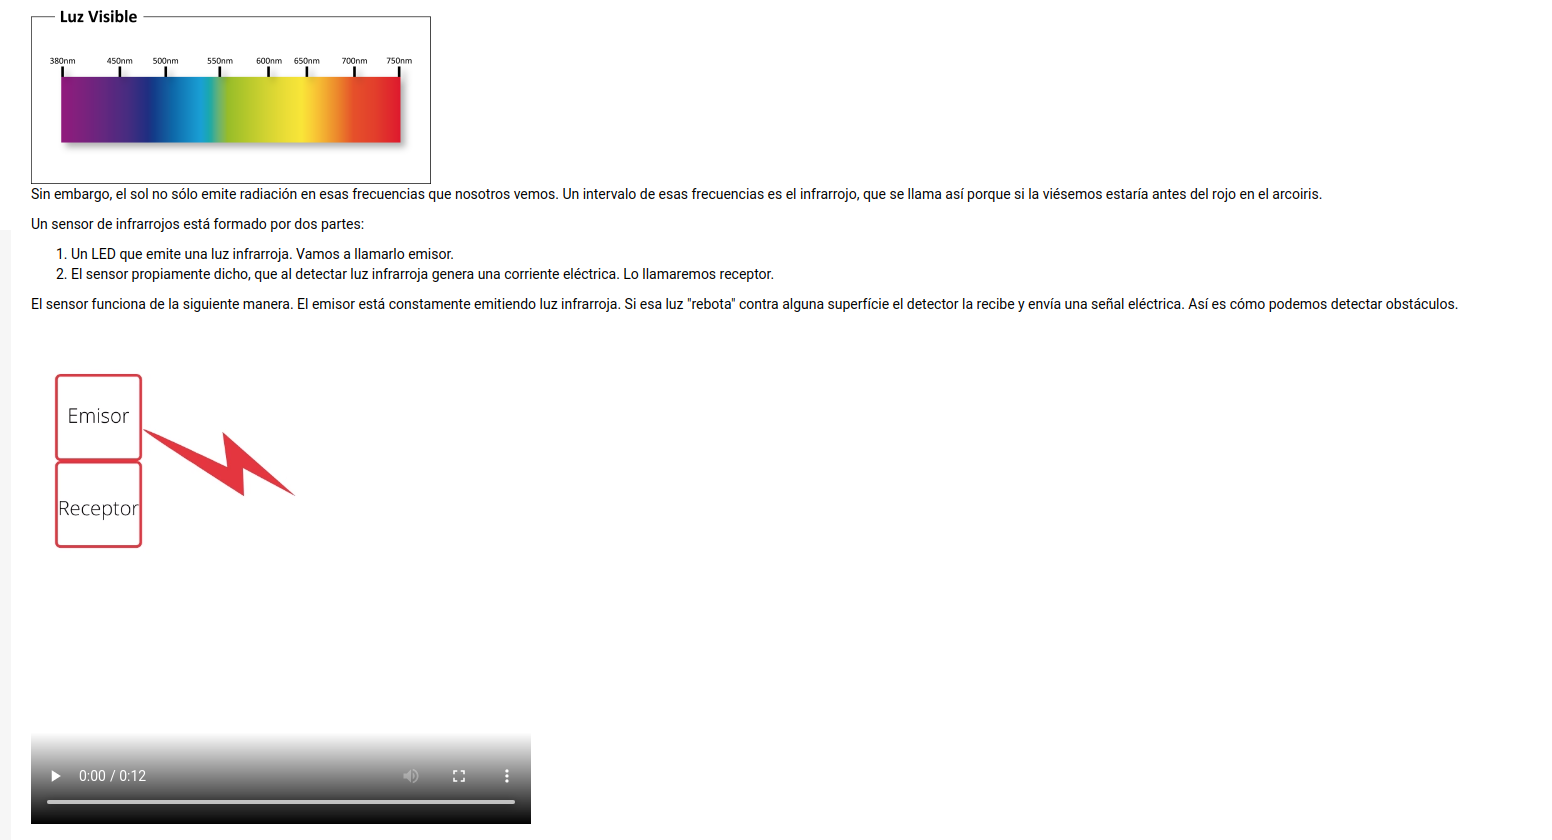
\includegraphics[width=1\textwidth, height=0.4\textwidth]{chapters/images/teoriag2.png}
    \caption{Teoría infrarrojos}
    \label{fig:my_label}
\end{figure}
\begin{figure}[H]
    \centering
    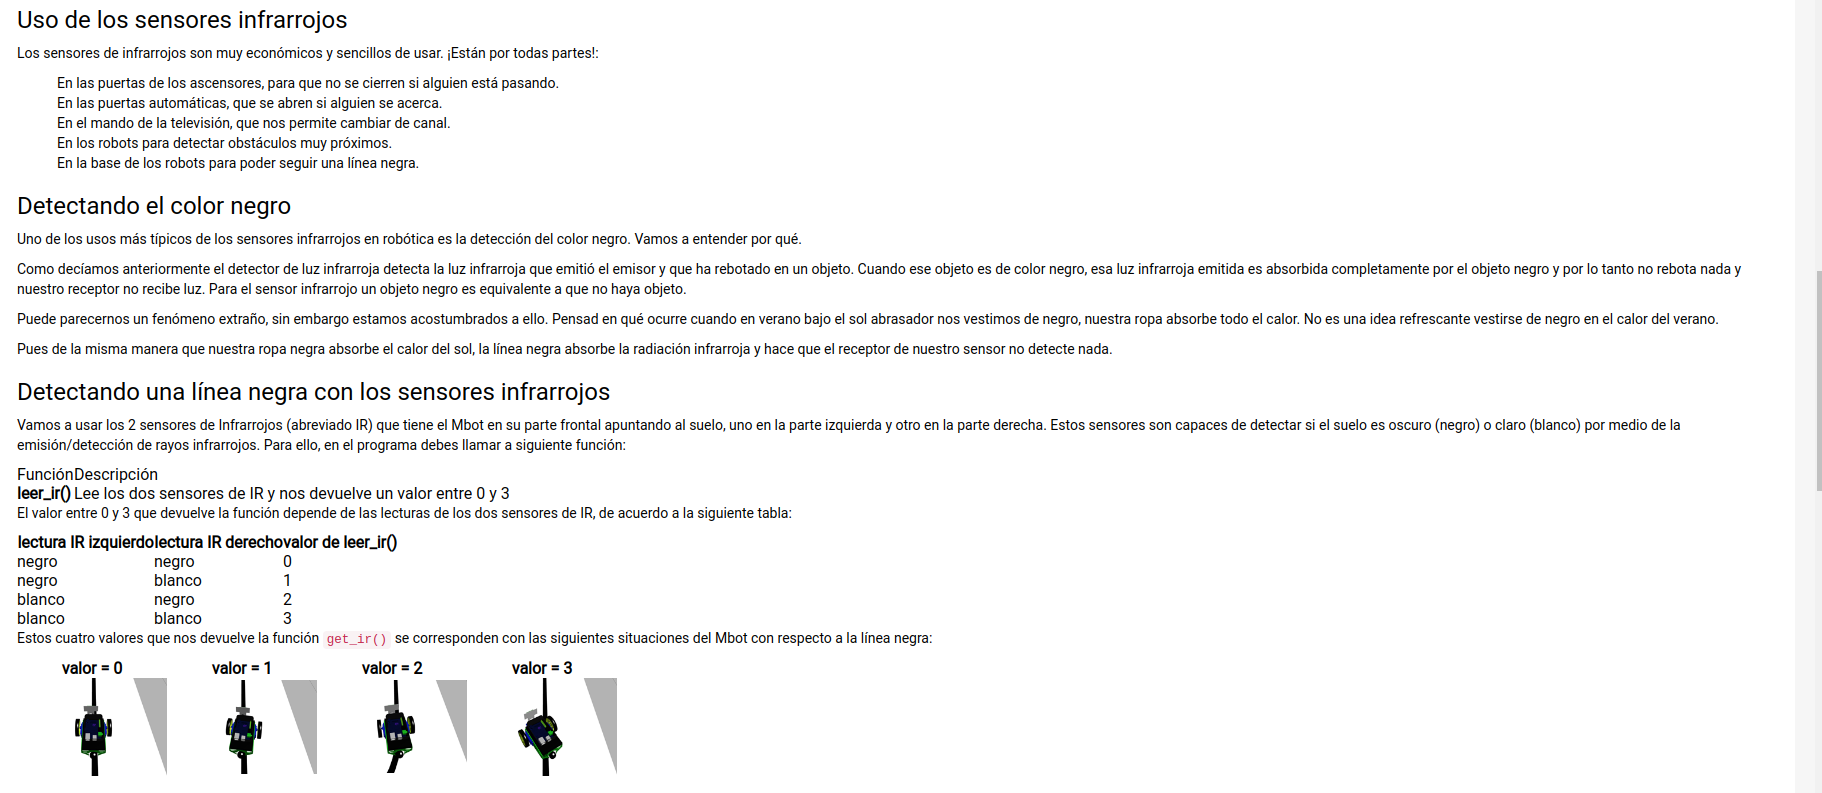
\includegraphics[width=1\textwidth, height=0.4\textwidth]{chapters/images/teoriag3.png}
    \caption{Teoría sensor infrarrojos}
    \label{fig:my_label}
\end{figure}

\begin{figure}[H]
    \centering
    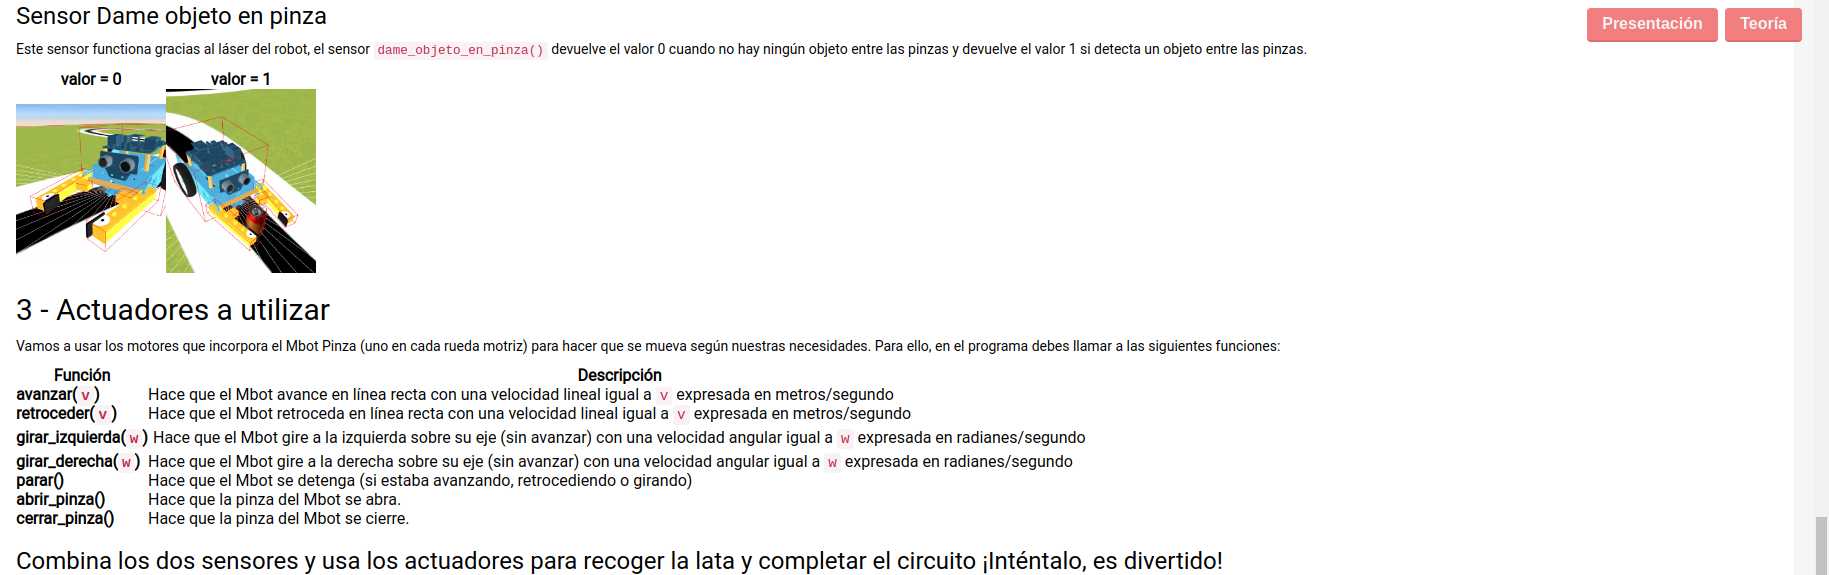
\includegraphics[width=1\textwidth, height=0.4\textwidth]{chapters/images/teoriag4python.png}
    \caption{Teroría sensores y actuadores en Python}
    \label{fig:my_label}
\end{figure}
\begin{figure}[H]
    \centering
    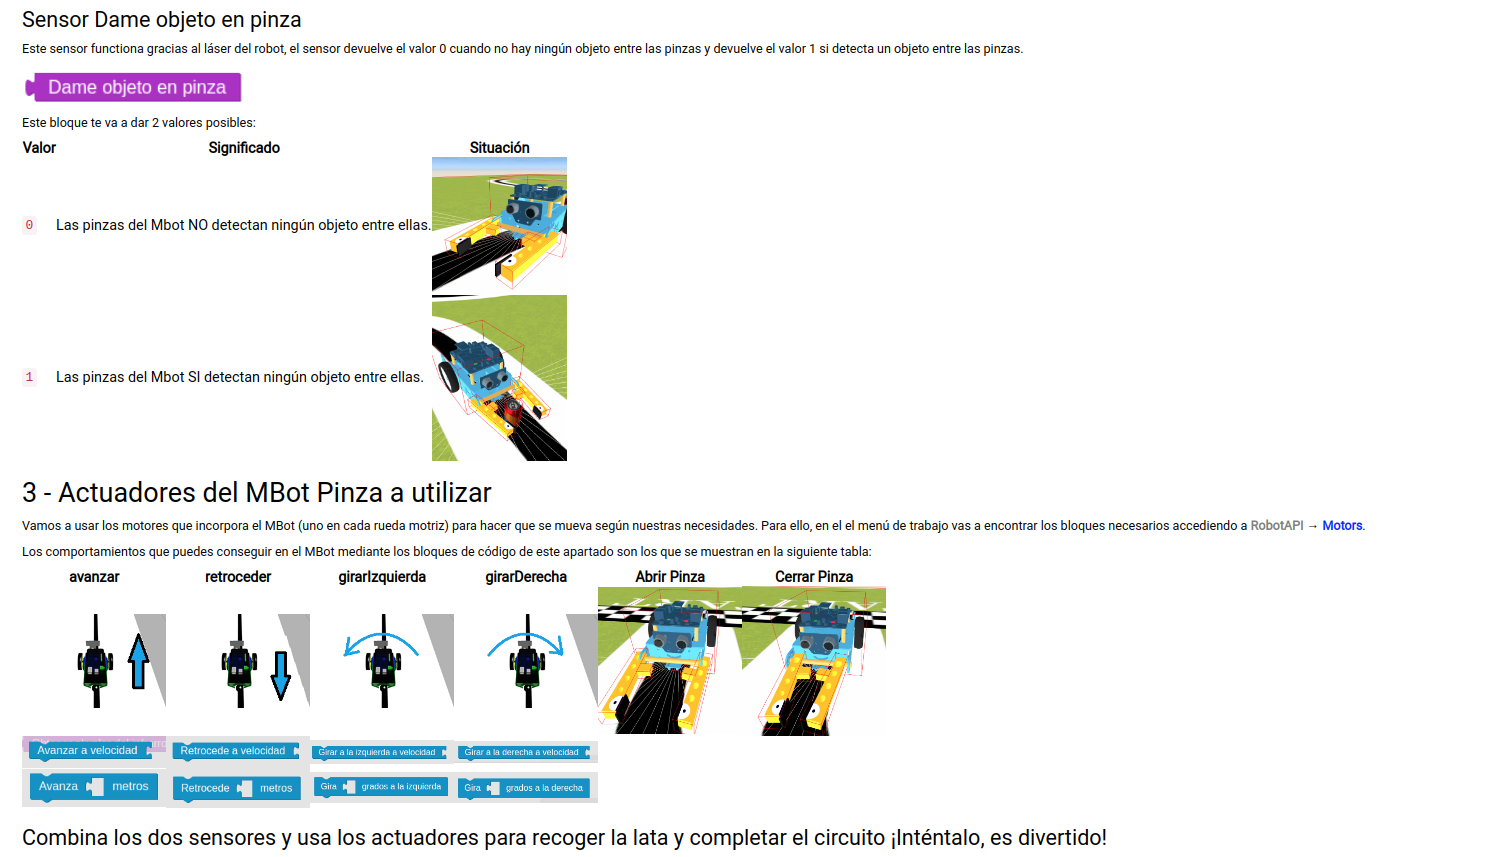
\includegraphics[width=1\textwidth, height=0.4\textwidth]{chapters/images/teoriag4scratch.png}
    \caption{Teroría sensores y actuadores en Python}
    \label{fig:my_label}
\end{figure}
\begin{figure}[H]
    \centering
    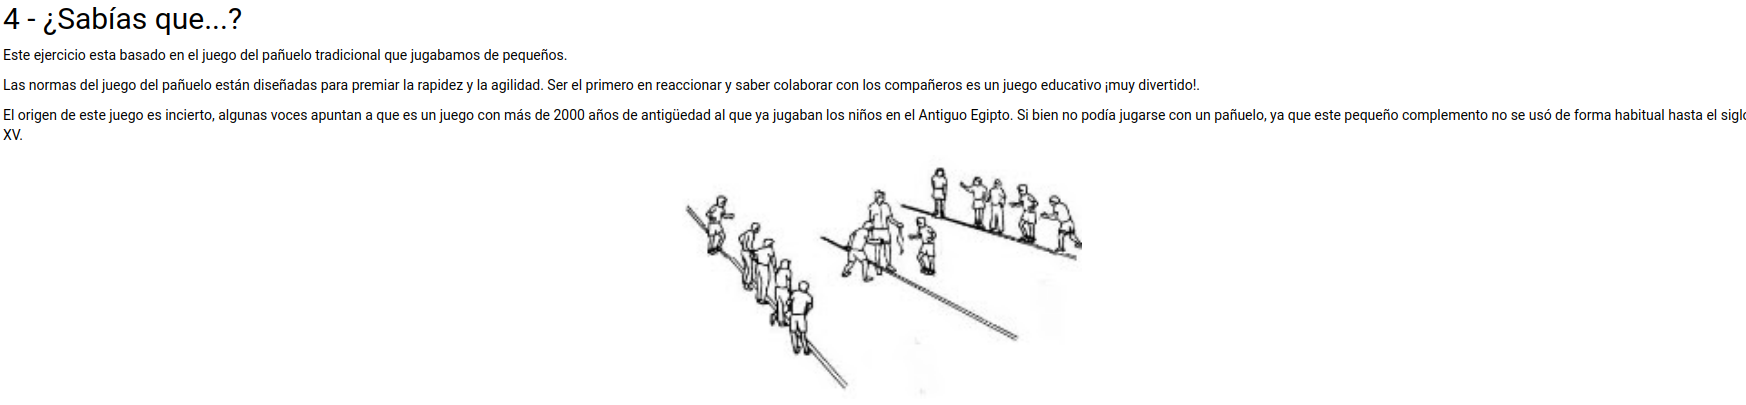
\includegraphics[width=1 \textwidth, height=0.27\textwidth]{chapters/images/teoriag5.png}
    \caption{¿Sabías que.. ?}
    \label{fig:my_label}
\end{figure}

La teoría se divide en 5 apartados, primero se hace una breve introducción del ejercicio y los objetivos que tiene que cumplir el alumno. En el primer punto se comenta qué se va a aprender en esta unidad. En el segundo punto se explica la teoría de los sensores que se van a utilizar, en este caso, son necesarios el sensor infrarrojos y el sensor dame objeto en pinza que se ha desarrollado en este trabajo. En el tercer punto se nombran los actuadores de movimiento, junto con  el abrir y cerrar de las pinzas necesarios para hacer el ejercicio y se indican las funciones y los bloques para poder utilizarlos en Python y en Scratch. Finalmente, el punto 4 trata de un ``¿Sabías que...?''  que cuenta datos curiosos sobre este antiguo juego.

\section{Modelos del mundo}
En este apartado se explica cómo se han creado los modelos de la lata y el circuito de este ejercicio.
El modelo 3D de la lata se creó con Blender (Figura 5.8 a). Para hacer el circuito se utilizó  GIMP, que es un programa de edición de imágenes gratuito y multiplataforma (versión 2.10), con él se diseñó la imagen .png del circuito (Figura 5.8 b) .
 
\begin{figure}[H]
  \begin{subfigure}[b]{0.5\textwidth}
  \centering
    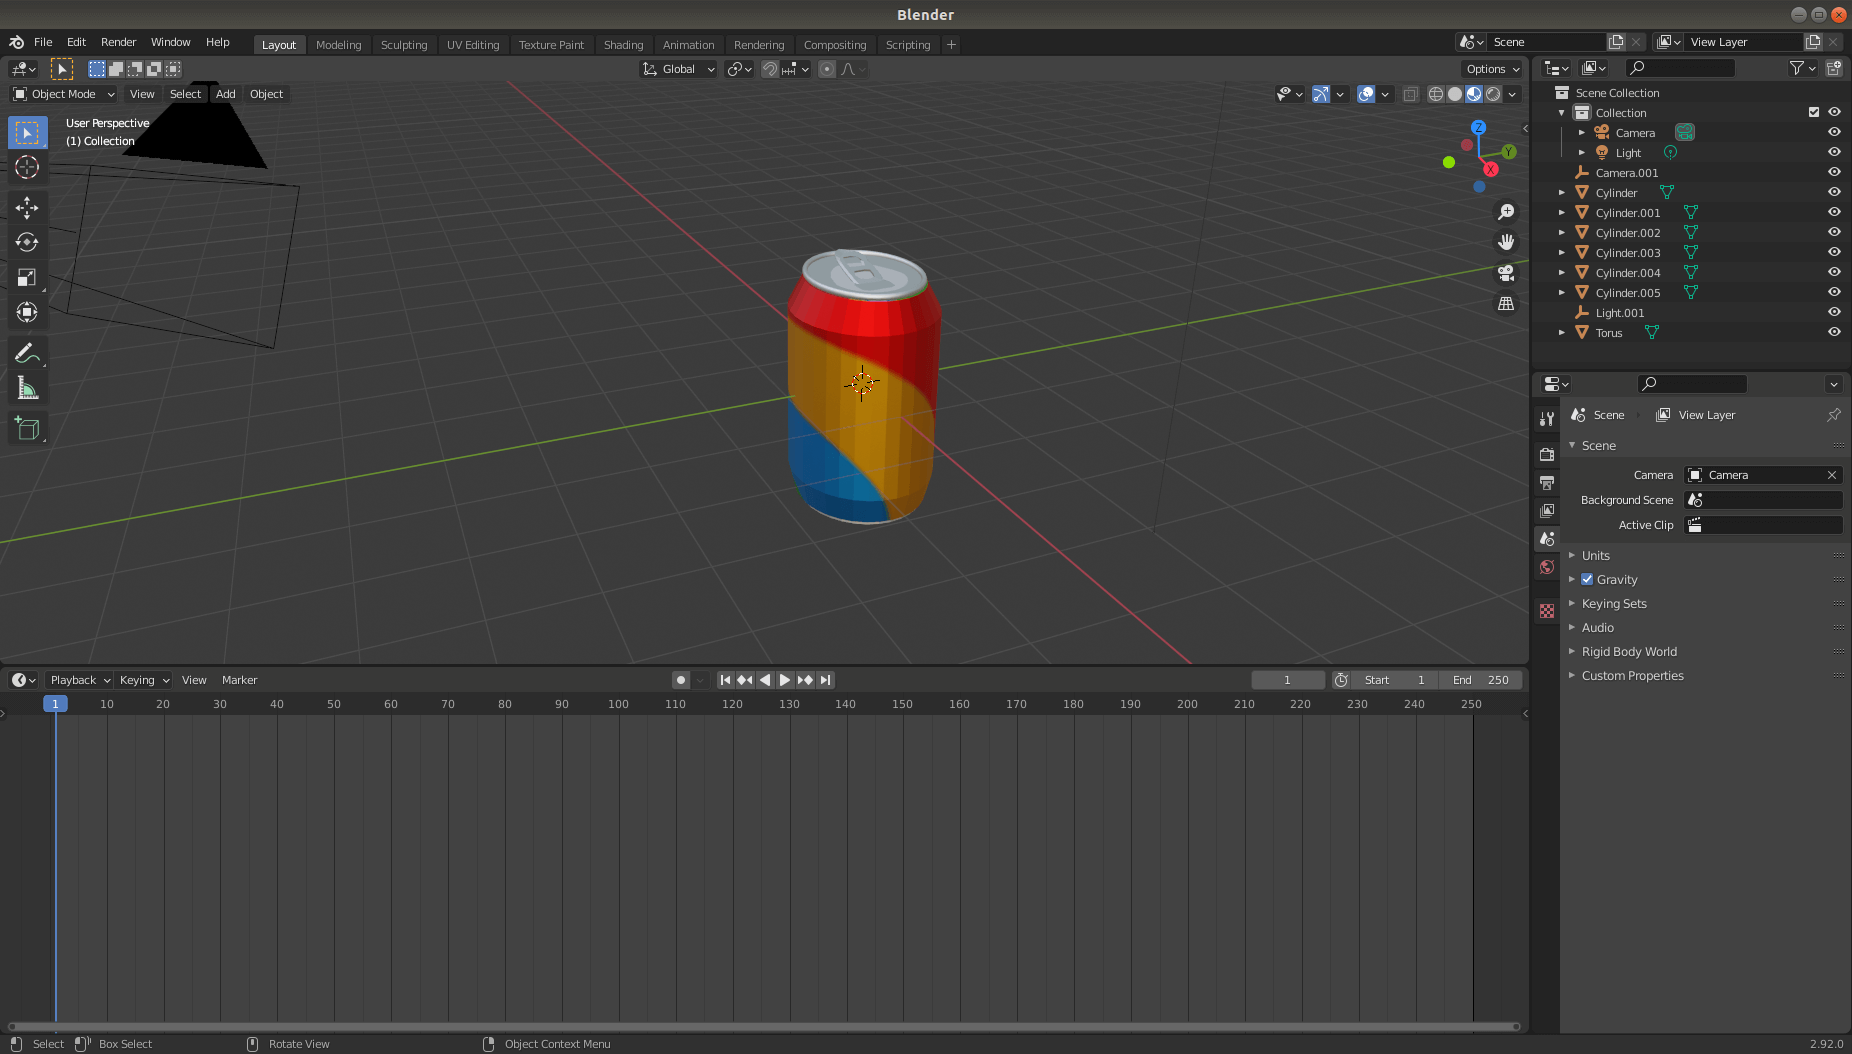
\includegraphics[width=1\textwidth, height=0.6\textwidth]{chapters/images/lata.png}
    \caption{Modelo lata}
    \label{fig:f1}
  \end{subfigure}
  \hfill
  \begin{subfigure}[b]{0.5\textwidth}
  \centering
     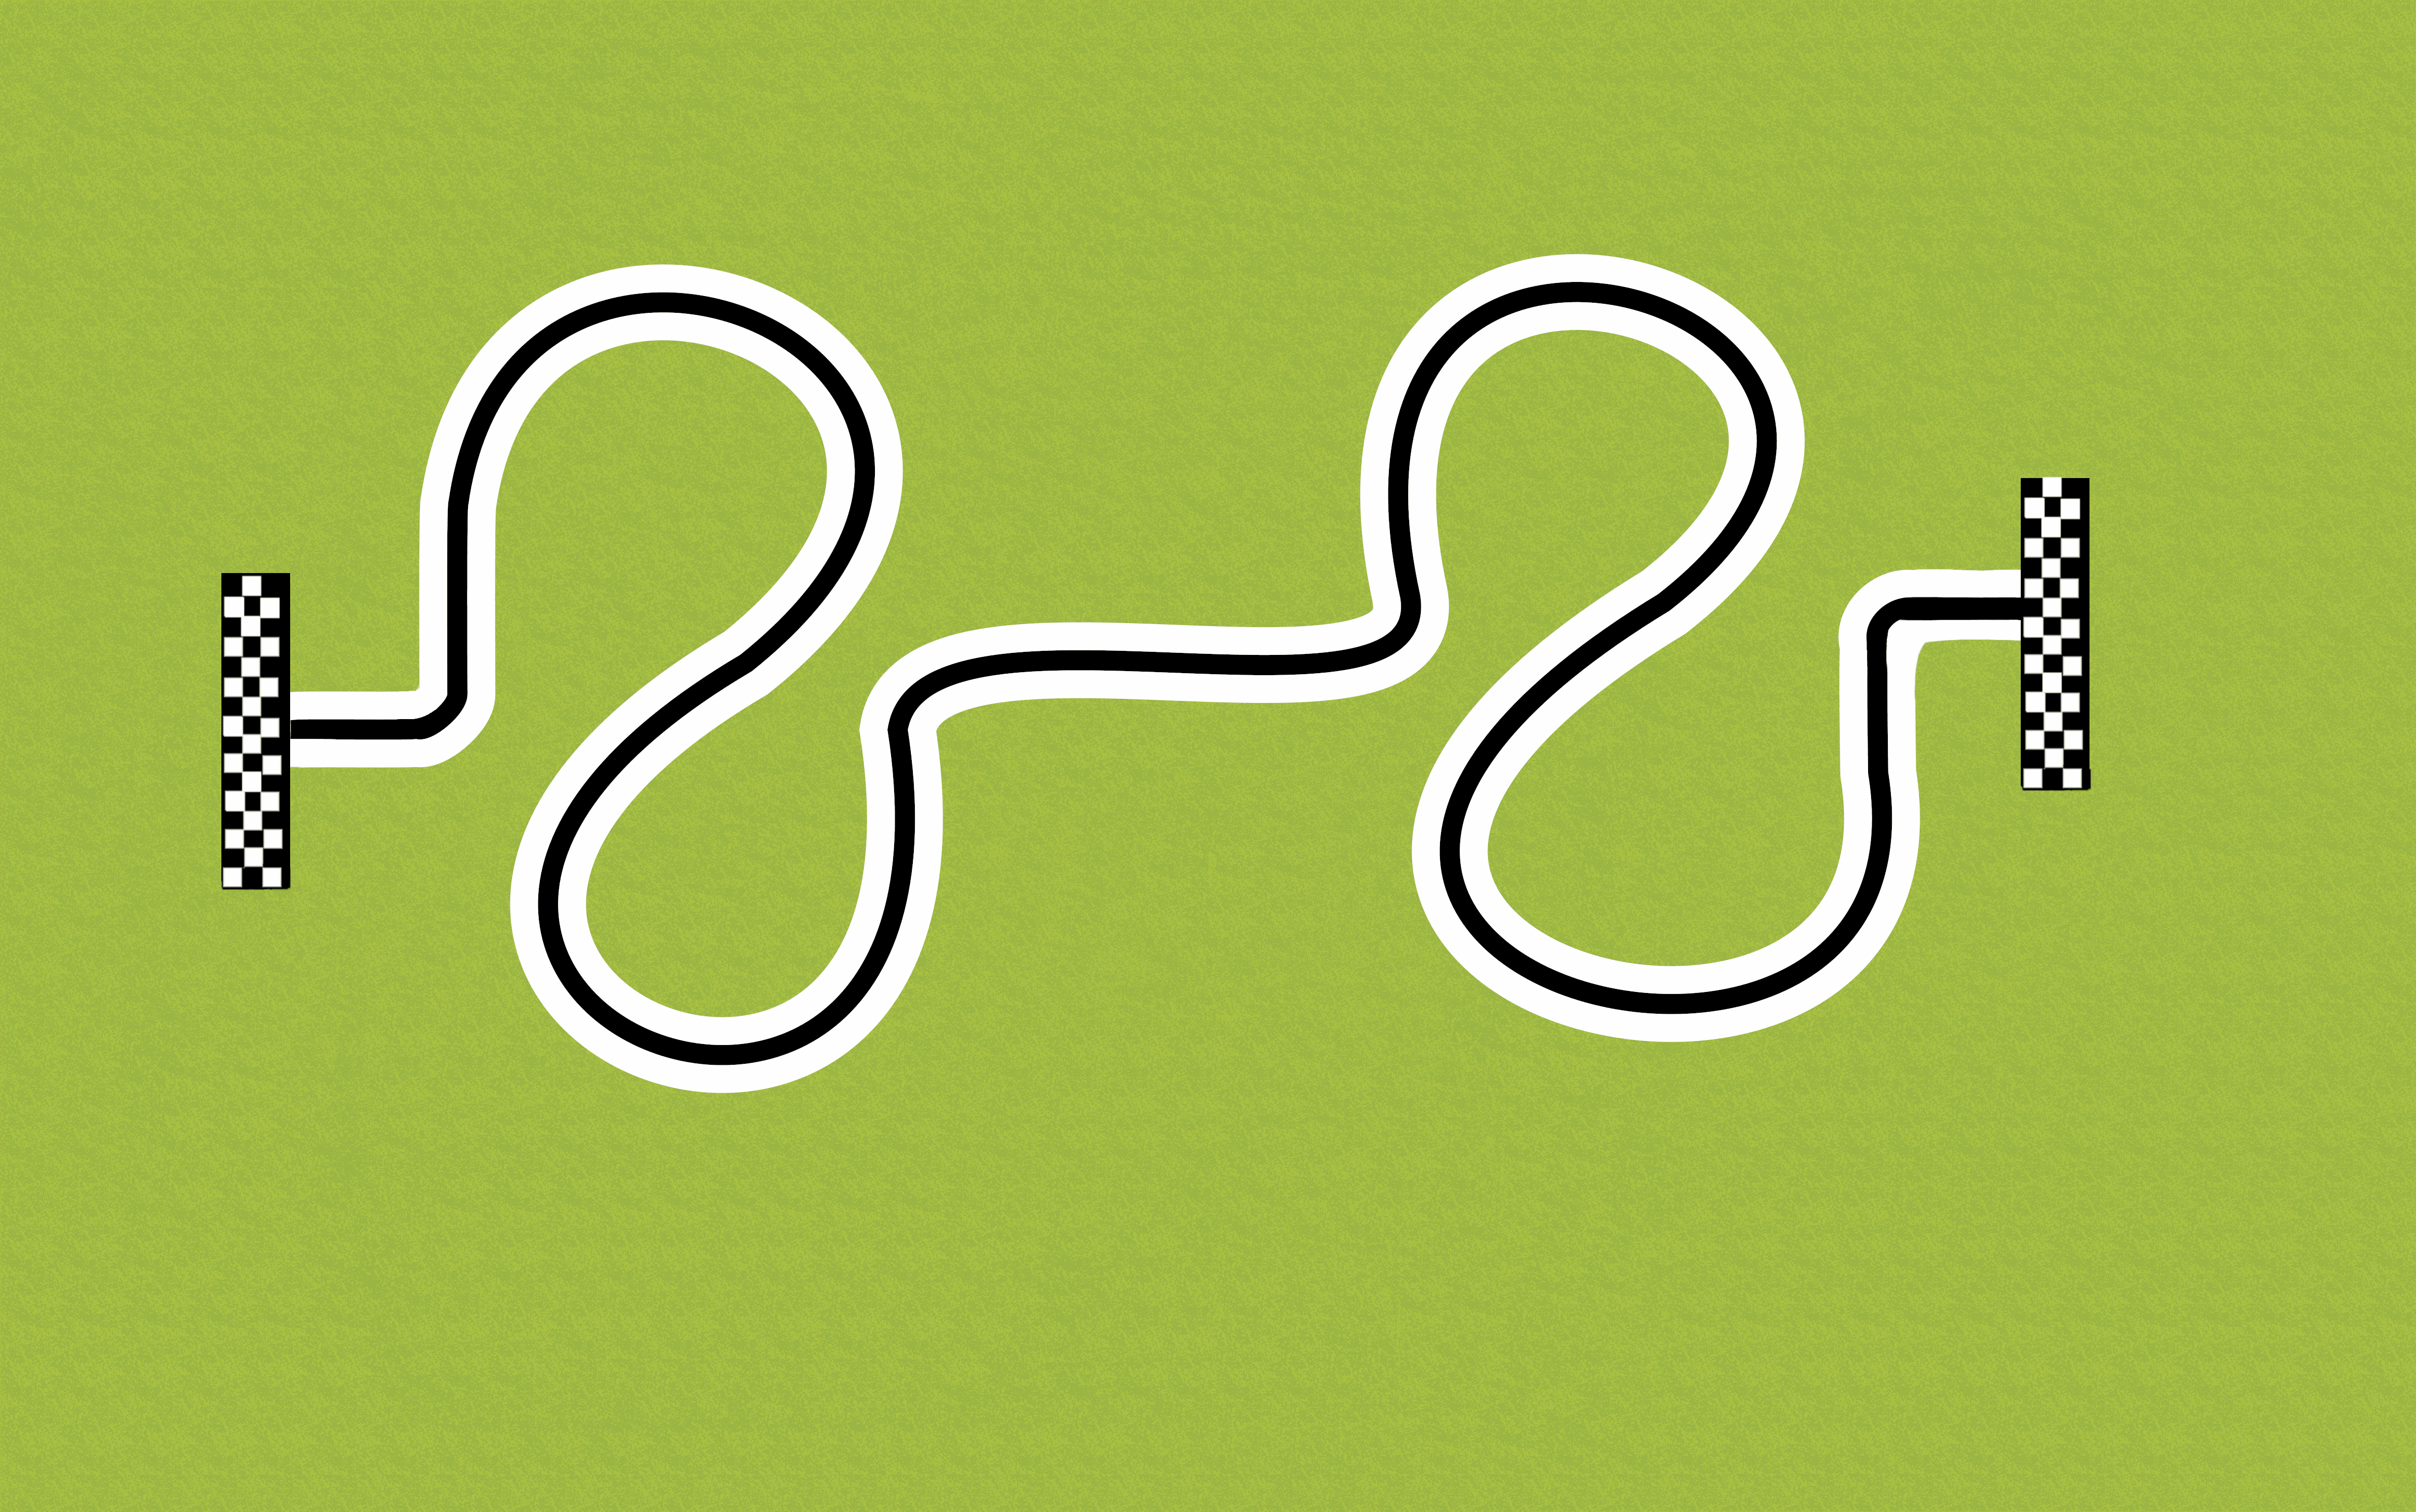
\includegraphics[width=1\textwidth, height=0.6\textwidth]{chapters/images/handkerchief.png}
     \caption{Circuito diseñado en GIMP del juego del pañuelo} 
    \label{fig:f2}
 
  \end{subfigure}
  \caption{Modelos en Blender}
\end{figure}
 
 
Los objetos se añadieron de la siguiente forma al fichero de configuración:
\begin{lstlisting}
 ...
 "assets": [
    {
      "tag": "img",
      "attr": {
        "id": "ground",
        "alt": "Texture for the scene ground",
        "src": "/static/websim/assets/textures/handkerchief.png"
      }
    },
    {
      "tag": "a-asset-item",
      "attr": {
        "id": "model-pibot"
      }
    },
    {
      "tag": "a-asset-item",
      "attr": {
        "id": "model-can"
      }
    },
    ],
    
   "objects":[
 {
      "tag": "a-entity",
      "attr": {
        "id":"object",
        "gltf-model":"/static/websim/assets/models/can.gltf",
        "position": { "x":-2.25, "y":0.6, "z":-10.25},
        "rotation": { "x":0, "y":0, "z":0},
        "scale": { "x":0.3, "y":0.3, "z":0.3},
        "body":{"type": "dynamic", "mass": 20, "shape":"cylinder"},
        "class": "collidable"
      }
    },
    
    {
      "tag": "a-plane",
      "attr": {
        "static-body": {
          "mass": 100000
        },
        "position": { "x":0, "y":0, "z":-4 },
        "rotation": { "x":-90, "y":0, "z":0 },
        "width": "100",
        "height": "100",
        "src":"#ground"
      }
    },
    ]
 ...
 \end{lstlisting}

A la hora de crear la escena en el fichero de configuración de este ejercicio, se tuvo que añadir el atributo ``renderer":``colorManagement: true"  para que los colores en Websim fueran los mismos que se habían diseñado en Blender, sino los modelos se verían más oscuros. 

\begin{lstlisting}
"scene": {
    "id": "scene",
    "gravity": -9.8,
    "ground": "/static/websim/assets/textures/handkerchief.png",
    "sky": "/static/websim/assets/textures/sky.png",
    "background": "color: gray;",
    "inspector": "url: https://aframe.io/releases/0.4.0/aframe-inspector.min.js",
    "embedded": true,
    "physics": "debug: false; friction:0.0002",
    "renderer":"colorManagement: true"
  }, ...
 \end{lstlisting}


\section{Modelo robot con pinza}
En este apartado se va a explicar,  por un lado, el prototipo en A-Frame nativo hecho por Roberto Pérez, un colaborador de JdeRobot, y por otro, de cómo se ha creado finalmente el nuevo robot con pinzas.

\subsection{Antecedentes}
El prototipo existente en la plataforma estaba realizado en A-Frame nativo, (HTML5, JavaScript y la librería de A-Frame) sin Websim. Este primer prototipo cogía el modelo del Mbot que ya se usaba en Kibotics para algunos ejercicios y lo representaba en la escena. El robot se movía mediante eventos de teclado con JavaScript. 

Las pinzas eran dos ortoedros a los lados del robot. Estas pinzas estaban creadas con a-box y eran  independientes del robot. Con este prototipo se estudió el movimiento de las pinzas con respecto a la posición del robot. El código JavaScript era muy complejo y todos los objetos dependían de la actualización continua explícita de la posición. 
Se encontraron muchas dificultades a la hora de realizar los giros del robot con las pinzas, dado que éstas estaban definidas por el centro de masas y al rotar las pinzas había que hacerlo con funciones senoidales para que se movieran en concordancia con la rotación del robot. En la Figura 5.9 y en estos vídeos \footnote{https://www.youtube.com/watch?v=BpAujxcWx-Y}\footnote{https://www.youtube.com/watch?v=w5plHB\_4G7Y} se puede ver el prototipo y los problemas con el giro.

 \begin{figure}[H]
  \centering
 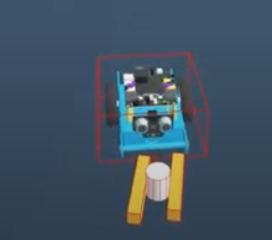
\includegraphics[width=0.40\textwidth]{chapters/images/prototipo.png}
  \caption{Prototipo robot con pinza en A-Frame nativo.}
\end{figure}

En este trabajo fin de grado el prototipo mencionado se ajustó y se llevó a Websim pero no funcionaba bien. Esta dependencia continua de la posición del robot con respecto a las pinzas y la lata con el cierre de las pinzas era muy compleja y muy poco realista. En este vídeo  \footnote{https://www.youtube.com/watch?v=eVM9n4mziTQ\&t=46s} se puede ver cómo era el funcionamiento en Websim con el JavaScript de este primer prototipo.  


\subsection{Modelo Mbot con pinzas}
La idea principal de este ejercicio era que el robot pudiera coger con las pinzas una lata de la forma más natural posible.
Para el robot base se usó el modelo del Mbot, ya teníamos su  modelo 3D en formato .gltf y para que fuera diferente a los anteriores que se usaban en la plataforma se cambió el color del robot desde Blender con tonos amarillos y azules (Figura 5.10). Se insertó en el fichero de configuración del ejercicio de la siguiente forma:

\begin{lstlisting}
 {
      "tag": "a-robot",
      "attr": {
        "id": "a-pibot",
        "gltf-model":"/static/websim/assets/models/mbot_base.gltf",
        "scale": { "x":25, "y":25, "z":25},
        "position": { "x":-35, "y":0.5, "z":-6},
        "rotation": { "x":0, "y":0, "z":0},
        "dynamic-body":{"mass": 1,"shape":"none"},
        "shape__main":{"shape": "box",
          "halfExtents": "0.055 0.04 0.05",
          "offset": "-0.025 0.04 0"
        }
      },
\end{lstlisting}

\begin{figure}[H]
  \centering
  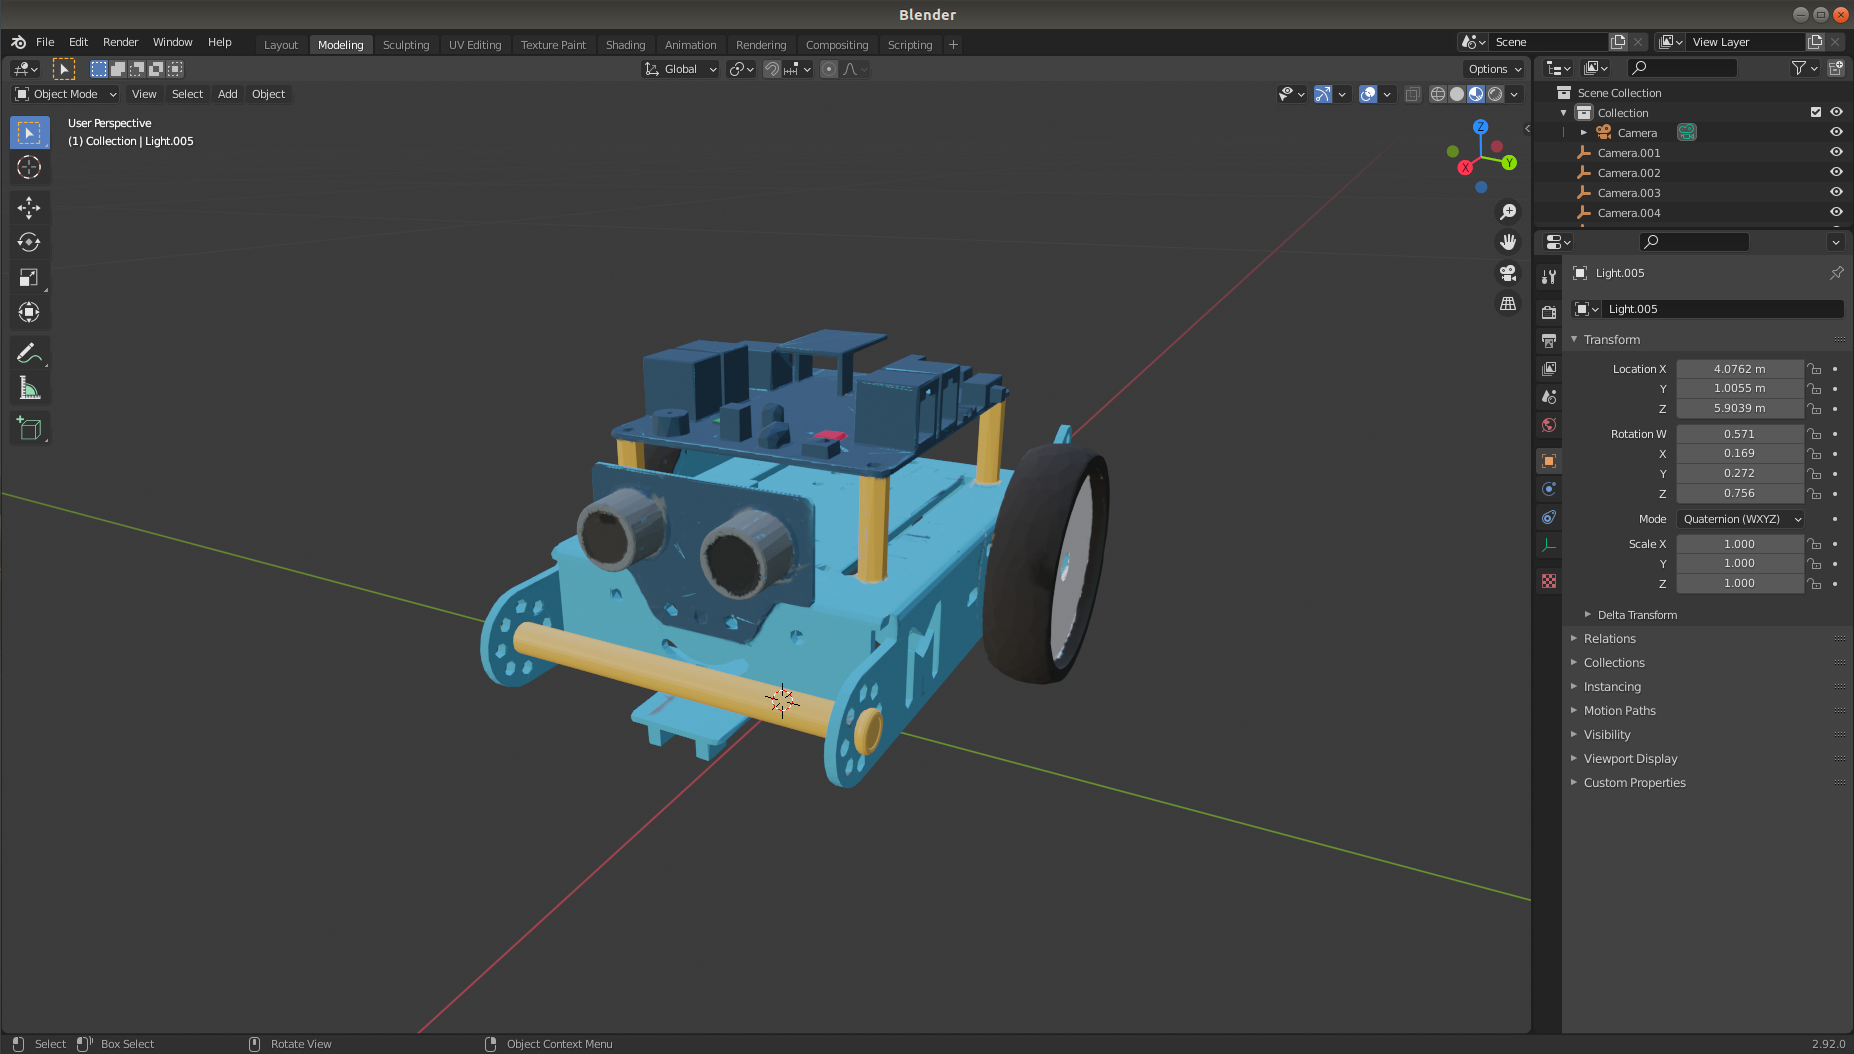
\includegraphics[width=0.6\textwidth]{chapters/images/mbotbase.png}
	\caption{Modelo Mbot cambiado de color}  
\end{figure}


Para las pinzas  primero se implementaron ortoedros gracias a la etiqueta  \textless box \textgreater de A-Frame. Pero finalmente se cambiaron por un modelo más moderno diseñado en Blender (Figura 5.10) .

\begin{figure}[H]
  \centering
    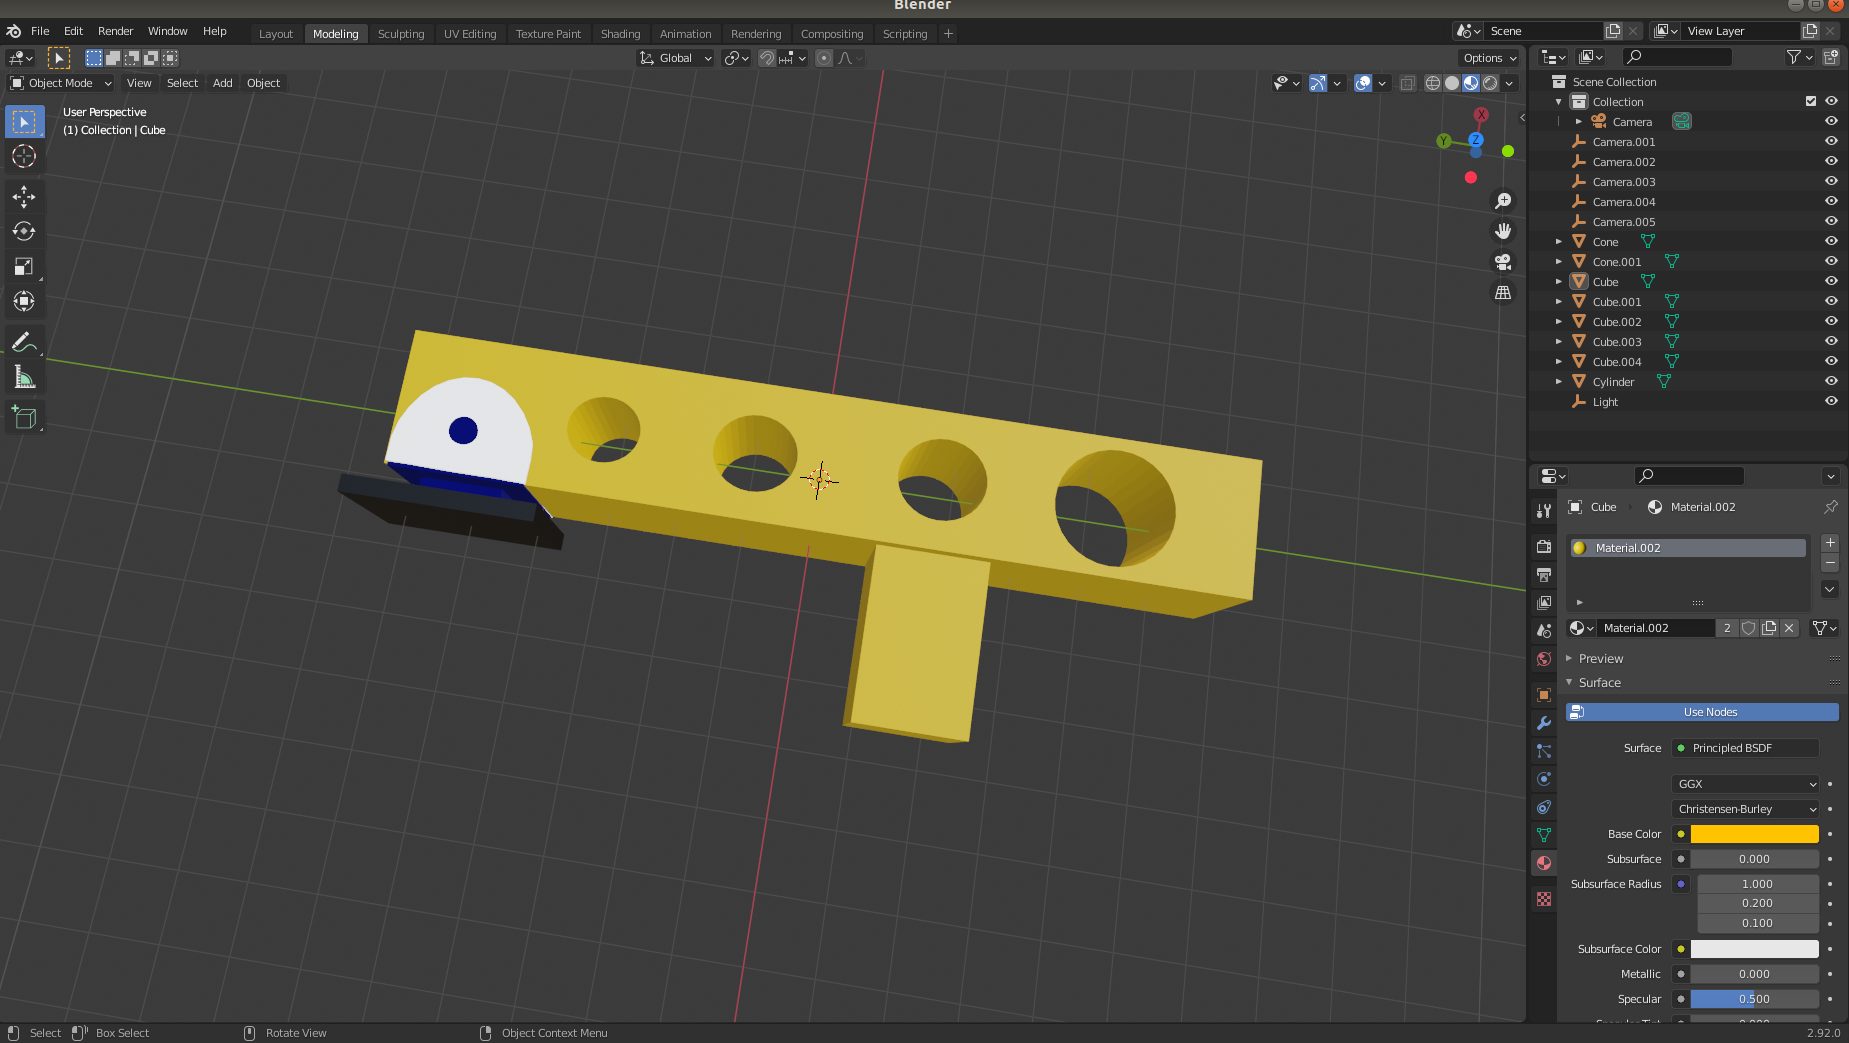
\includegraphics[width=0.6\textwidth]{chapters/images/pinza.png}
	\caption{Modelo Pinza}    
\end{figure}


Las pinzas tenían que ser dependientes del robot para que su movimiento y los giros fueran coherentes. 
Para conseguir esta dependencia de las pinzas con el robot, desde el fichero de configuración, las pinzas se definieron como objetos hijos (\textit{childs}) del objeto robot base (el Mbot). De esta forma las pinzas y el robot forman un mismo objeto y se mueven a la vez.

\begin{lstlisting}
   {
      "tag": "a-robot",
      "attr": {
        "id": "a-pibot",
        "gltf-model":"/static/websim/assets/models/mbot_base.gltf",
        "scale": { "x":25, "y":25, "z":25},
        "position": { "x":-35, "y":0.5, "z":-6},
        "rotation": { "x":0, "y":0, "z":0},
        "dynamic-body":{"mass": 1,"shape":"none"},
        "shape__main":{"shape": "box",
                                   "halfExtents": "0.055 0.04 0.05",
                                   "offset": "-0.025 0.04 0"
        }
      },
      
      "childs": [
            {
              "tag": "a-entity",
              "attr": {
                "id":"gripper-left",
		          "gltf-model":"/static/websim/assets/models/gripper.gltf",
                  "position": { "x":-0.033, "y":0, "z":-0.05},
                  "scale": { "x":0.005, "y":0.005, "z":0.006},
                  "rotation": { "x": 0, "y":-8, "z":180},
                  "body":{"type": "static", "mass": 1, "shape":"none"},
                  "shape__main":{"shape": "box",
                     "halfExtents": "1.5 1.5 6.5",
                                 "offset": "0 0 0"},
                  "shape__handle":{"shape": "box",
                           "halfExtents": "1.5 1 1",
                           "offset": "-2.2 -0.2 1.75"}
              }
            },
            {
              "tag": "a-box",

              "attr": {
                "id":"gripper-right",
		        "gltf-model":"/static/websim/assets/models/gripper.gltf",
                "position": { "x":0.033, "y":0, "z":-0.05},
                "scale": { "x":0.005, "y":0.005, "z":0.006},
                "rotation": { "x": 0, "y":8, "z":0},
                "body":{"type": "static", "mass": 1, "shape":"none"},
                "shape__main":{"shape": "box",
			       "halfExtents": "1.5 1.5 6.5",
                               "offset": "0 0 0"},
		        "shape__handle":{"shape": "box",
                         "halfExtents": "1.5 1 1",
                         "offset": "-2.2 -0.2 1.75"}
              }
              
            },
         
      ]
    },
    
\end{lstlisting}

A continuación se explica cómo se han ajustado los atributos de los objetos mostrados en el código anterior.

En A-Frame existen dos tipos de cuerpos: \textit{dynamic-body y static-body}. Un objeto con \textit{dynamic-body}  se mueve libremente. Los cuerpos dinámicos tienen masa, chocan con otros objetos, rebotan o se ralentizan durante las colisiones y caen si la gravedad está habilitada.
Los cuerpos estáticos son objetos animados o de posición fija. Otros objetos pueden chocar con cuerpos estáticos, pero los cuerpos estáticos en sí mismos no se ven afectados por la gravedad ni las colisiones.

El robot se definió como un cuerpo dinámico mientras que las palas de las pinzas eran cuerpos estáticos, de esta forma, las palas pueden estar elevadas del suelo y no les afecta  radicalmente las colisiones que pueda tener con la lata a la hora de cerrarse. La lata en cambio es un objeto dinámico.

La malla de colisión se define por \textit{shape\_main y shape\_handle}. En el atributo \textit{body} se pone ``shape: none'' para poder ajustar la malla de colisión que viene por defecto con \textit{shape\_main y shape\_handle} .
\textit{Shape\_main} es la malla de colisión principal en la que se puede elegir la forma, \textit{shape}, lo que ocupa \textit{halfExtents} y se puede desplazar del centro del objeto \textit{offset}. Esto nos permite hacer la malla de colisión más grande o más pequeña que las dimensiones de nuestro objeto. \textit{ Shape\_handle} nos permite añadir una malla de colisión extra independientemente de si dentro de ese  objeto hay otro objeto o no. Esta malla de colisión extra se define respecto a la malla de colisión \textit{shape\_ main}. Ambas mallas de colisión dependerán de la posición del objeto y se moverán lo mismo que él.

La malla de colisión extra se usó para la parte cúbica que tiene la parte central del modelo de la pinza usando la forma  \textit{ ``shape'' : ``box''},  ajustando  la posición y dimensiones del cubo, mientras que la malla de colisión principal se asignó a la parte del modelo con forma de ortoedro, también con \textit{ ``shape'' : ``box''} pero ajustándolo a las medidas del ortoedro.

En la Figura  5.12 se muestra el Mbot con pinzas con sus modelos, físicas y sus 5 mallas de colisión.

 \begin{figure}[H]
  \centering
 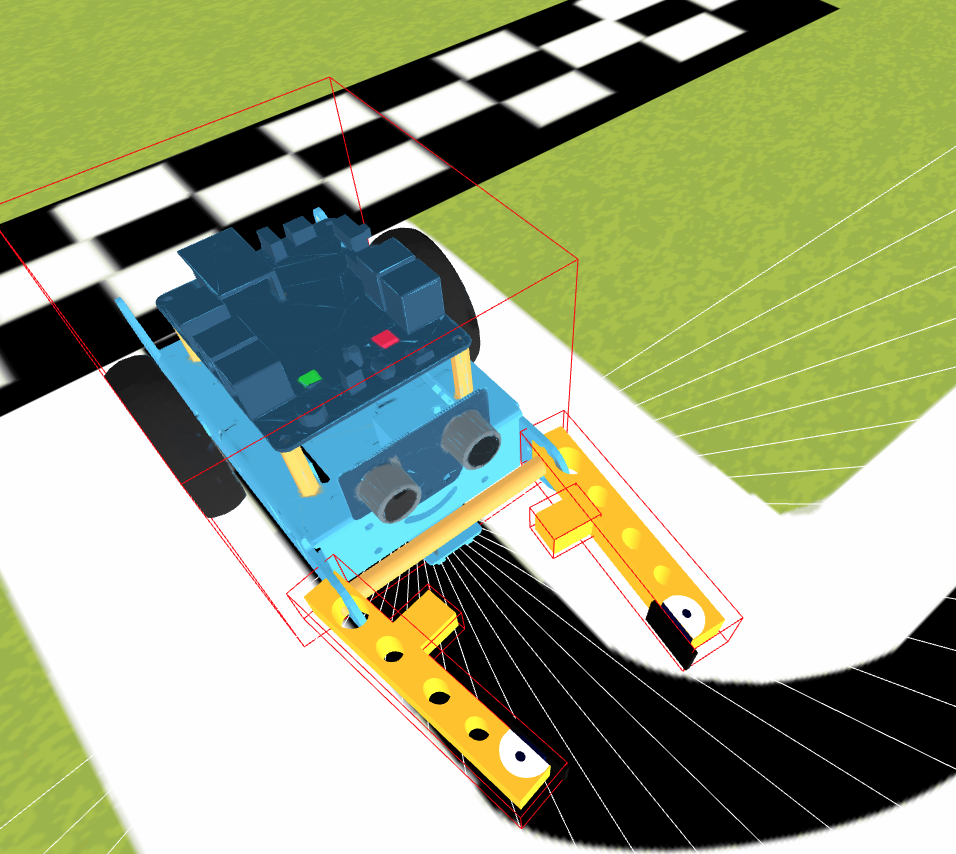
\includegraphics[width=0.5\textwidth, height=0.4\textwidth]{chapters/images/mallas.png}
  \caption{Mallas de colisión del robot}
\end{figure}

Los usuarios tienen que programar el Mbot para que éste abra y cierre las pinzas cuando la lata esté cerca. Para ello, implementaron las funciones \textit{closeGripper(), openGripper() y getObjectInGripper()} en JavaScript para luego crear los bloques y funciones respectivas en Scratch y Python, con las que los usuarios puedan manejar todas las operaciones del robot. 
 
En Scracth se crearon nuevos bloques en los Motores : \textit{Abrir pinza, Cerrar Pinza y Dame objeto en pinza}.
En Python  se crearon las nuevas funciones: \textit{HAL.abrir\_pinza(), HAL.cerrar\_pinza() y  HAL.dame\_objeto\_en\_pinza()} que en el fondo todas ellas llaman las funciones JavaScript  del siguiente código para mover las pinzas y obtener la distancia entre la lata y el robot.
 
\begin{lstlisting}
export async function closeGripper() {

    let thread = getThread(this.myRobotID);
    thread.blocking_instruction = true;
    let gripperLeft = document.querySelector("#gripper-left")
    let gripperLeftPos = gripperLeft.object3D.position
    let gripperRight = document.querySelector("#gripper-right")
    let gripperRightPos = gripperRight.object3D.position
    let val = 0.025
    while (getThread(this.myRobotID).status !== "RELOADING" && gripperLeftPos.x < -0.020 && gripperRightPos.x > 0.020) {
        val = val - 0.001
        await document.querySelector("#gripper-left").setAttribute('position', {x: -val, y:0 , z: -0.05})
        await document.querySelector("#gripper-right").setAttribute('position', {x: val, y:0 , z: -0.05})
        await this.sleep(0.2);
    }
    thread.blocking_instruction = false;
}

export function getObjectInGripper() {
    let distance = this.getDistance();
    if (distance < 1.5) {
        return 1;
    } else {
        return 0;
    }
}

export async function openGripper() {
    await document.querySelector("#gripper-left").setAttribute('position', {x: -0.030, y:0 , z: -0.05})
    await document.querySelector("#gripper-right").setAttribute('position', {x: 0.030, y:0 , z: -0.05})

}
\end{lstlisting}


Una vez creado el robot y las funciones necesarias, se estudió la posibilidad de que ajustando  las mallas de colisión de las pinzas se pudiera atrapar una lata con la fuerza que ejercieran al cerrarse. 
Las mallas de colisión son las líneas rojas que delimitan el entorno de un objeto y permiten definir una forma física alrededor de modelos personalizados. Esto hace que funcionen mejor y se comporten con mayor realismo.

El cerrar las pinzas de esta forma,  la lata colisionaba con las mallas de colisión de las pinzas pero no se quedaba atrapada. Para solucionar ésto, se rotaron las pinzas 8 grados en el eje y. También se ajustaron las físicas del mundo para que el robot pudiera arrastrar la lata sin problemas por el escenario. En la Figura 5.13 podemos ver cómo eran las pinzas sin rotar y con ortoedros y las nuevas pinzas con el modelo de Blender rotado 8 grados que finalmente se utilizó.


\begin{figure}[H]
  \begin{subfigure}[b]{0.5\textwidth}
  \centering
    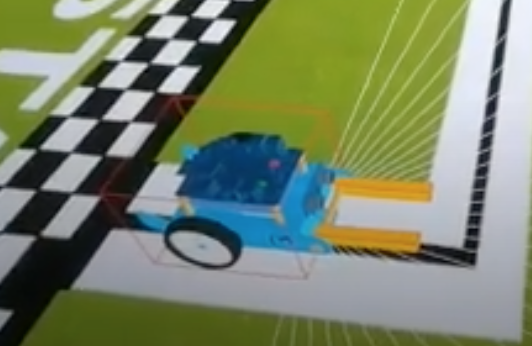
\includegraphics[width=0.8\textwidth, height=0.5\textwidth]{chapters/images/pinzarecta.png}
    \caption{Primeras pinzas con ortoedros rectas}
    \label{fig:f1}
  \end{subfigure}
  \hfill
  \begin{subfigure}[b]{0.5\textwidth}
  \centering
    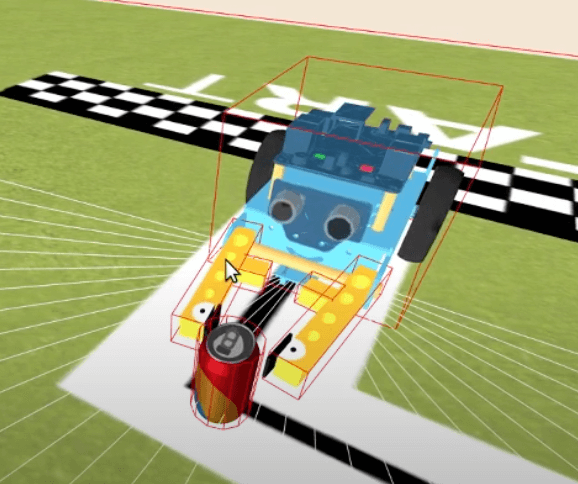
\includegraphics[width=0.8\textwidth, height=0.5\textwidth]{chapters/images/pinzaok.png}
	\caption{Pinzas rotadas 8 grados}    
    \label{fig:f2}
 
  \end{subfigure}
  \caption{Robot Mbot con pinzas}
\end{figure}

\section{Evaluador automático}

Por último se añadió un evaluador automático para mostrar el porcentaje del circuito recorrido con puntos de control y unos iconos para indicar que la lata está cogida o no. Esto se hizo en un fichero .js que se importa al ejercicio llamado gripper\_evaluator.js. En la Figura 5.14 se muestra la visualización del evaluador. En el siguiente código se puede ver cómo se ha implementado la comprobación de los puntos de control y si el robot coge la lata o no.


\begin{lstlisting}
  var checkpoints= [[-32,0,-6],[-31,0,-11], [-31,0,-17], [-30,0,-28],
                  [-27,0,-32], [-22,0,-34], [-19,0,-33],
                  [-17,0,-32], [-15,0,-28], [-14,0,-24],
                  [-14,0,-20],[-15,0,-16], [-18,0,-12],
                  [-24,0,-4],[-27,0,2],[-27,0,6],
                  [-26,0,12],[-18,0,16],[-13,0,8],
                  [-12,0,0],[-13,0,-5],[-8,0,-10],
                  [-5,0,-10],[-4,0,-10], [-5,0,-10],
		         [-8,0,-10],[-13,0,-5],[-12,0,0],
		         [-13,0,8],[-18,0,16],[-26,0,12],
		         [-27,0,6],[-27,0,2],[-24,0,-4],
		         [-18,0,-12],[-15,0,-16],[-14,0,-20],
		         [-14,0,-24],[-15,0,-28],[-17,0,-32],
		         [-19,0,-33],[-22,0,-34],[-27,0,-32], 
		         [-30,0,-28],[-31,0,-17],[-31,0,-11],
   		         [-32,0,-6],[-37,0,-6]
		 
];

  let robot = Websim.simulation.getHalAPI(robID);
   var x = Math.round(robot.getPosition().x)
   var z = Math.round(robot.getPosition().z)
   var element = document.getElementById("a-car1bar");
   var totalpuntuation = document.getElementById("totalpuntuation");
   var status = false;

   var can = document.getElementById('object')
   var canx = can.getAttribute('position').x
   var canz = can.getAttribute('position').z
   var takencan_distance = Math.sqrt(Math.pow((canx-x), 2)+Math.pow((canz-z), 2));
   if (takencan_distance <= 2.5){
    extrapoint.innerHTML= "&#x1f3c5 &#x2728";
   }else{
    extrapoint.innerHTML= "";
   }
   
   var d = Math.sqrt(Math.pow((checkpoints[n][0]-x), 2)+Math.pow((checkpoints[n][2]-z), 2));
   var d1 = Math.sqrt(Math.pow((checkpoints[n][0]+1-x), 2)+Math.pow((checkpoints[n][2]+1-z), 2));
   var d2 = Math.sqrt(Math.pow((checkpoints[n][0]-1-x), 2)+Math.pow((checkpoints[n][2]-1-z), 2));
   var d3 = Math.sqrt(Math.pow((checkpoints[n][0]+1-x), 2)+Math.pow((checkpoints[n][2]-1-z), 2));
   var d4 = Math.sqrt(Math.pow((checkpoints[n][0]-1-x), 2)+Math.pow((checkpoints[n][2]+1-z), 2));
	
	if (d <= 1 || d1 <= 1 || d2 <= 1 || d3 <= 1 || d4 <= 1){
	       n+=1
	       if(n >= 48){
		   if (takencan_distance <= 2.5){
		       totalpuntuation.innerHTML=100;
		   }
		   status = true;
		   element.style.width = 100 + '%';
		   element.innerHTML = 100 + '%';
	     }
	   }
	  
	  var completed = Math.round(n/checkpoints.length*100)
	  
	  if (n!==48){
	    element.style.width = Math.round(completed) + '%';
	    element.innerHTML = Math.round(completed) + '%';
	    totalpuntuation.innerHTML=Math.round(completed*0.66);
	    if (takencan_distance <= 2.5){
		totalpuntuation.innerHTML=Math.round(completed*0.66)+14;
	    }
	  }
    
\end{lstlisting}

Los puntos de control están repartidos por toda la mitad del circuito que es el recorrido que tiene que hacer el robot. Los puntos se van comparando uno a uno, de modo que si no ha pasado por el primer punto y el robot pasa por el segundo, no se tiene en cuenta, porque no ha recorrido el circuito de forma correcta. Esto se ha realizado con la distancia euclídea, si el robot se encuentra en un radio cercano al punto de control que le corresponda del circuito y se ha pasado por los anteriores, se aumenta el porcetaje de circuito recorrido, sino no.

Cuando la lata está entre las pinzas se muestra una medalla y unas estrellas. Esto se ha realizado también con la distancia euclídea, donde calculamos la distancia entre el robot y la lata y si es menor o igual a 2'5 se añade esa puntuación extra.

En la Figura 5.14, podemos ver que el robot a recorrido una parte del circuito bien pero no lo ha hecho correctamente, debería tener al rededor del  50\% de circuito recorrido. En cambio ha cogido la lata por eso se muestran los iconos.

 \begin{figure}[H]
  \centering
 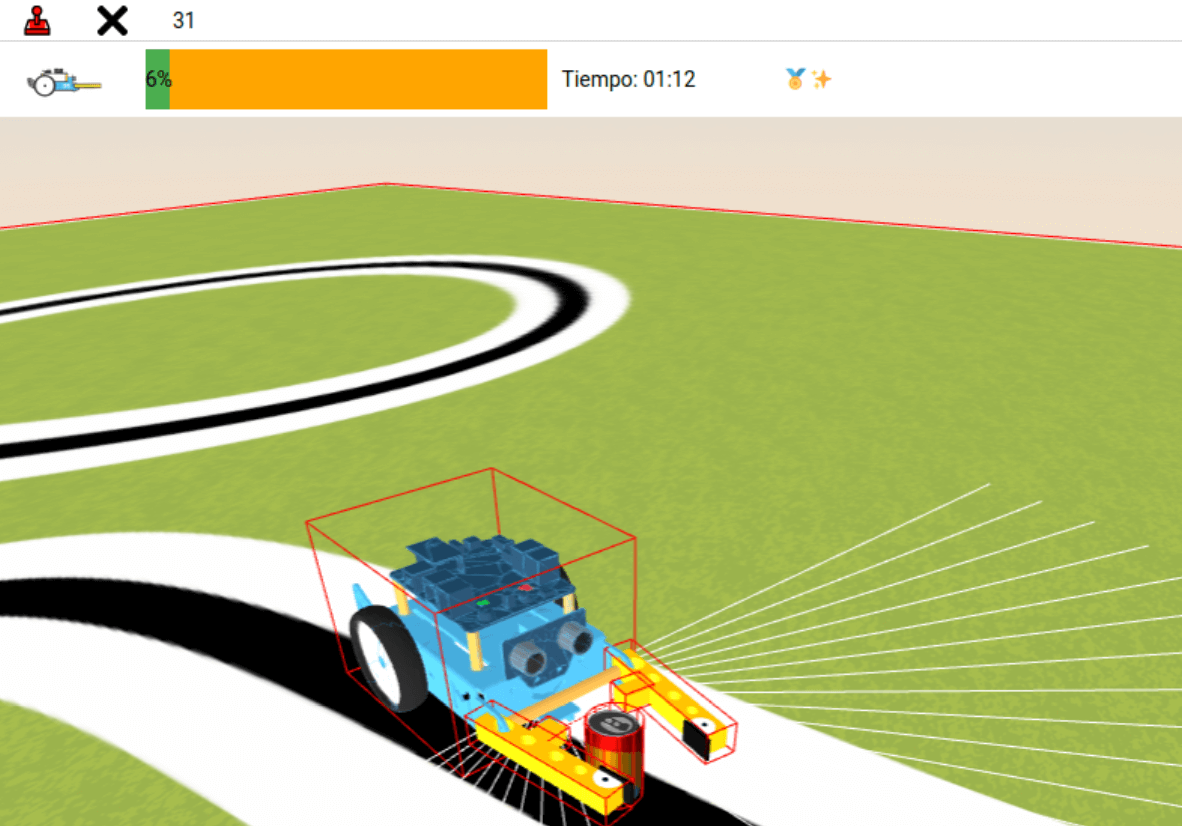
\includegraphics[width=0.75\textwidth, height=0.45\textwidth]{chapters/images/evaluadorpinza.png}
  \caption{Evaluador automático del juego del pañuelo}
\end{figure}


\section{Solución de referencia}
Este ejercicio se puede resolver de muchas formas, unas posibles soluciones son las que se muestran en la Figura 5.15 para Python y  en la Figura 5.16 para Scratch. 
En estas soluciones reflejan el código necesario para hacer un sigue líneas con el sensor de infrarrojos que dependiendo de su valor, el robot avanzará, girará a la izquierda o a la derecha hasta llegar a la lata. Con el sensor \textit{Dame objeto en pinza o HAL.dame\_objeto\_en\_pinza)} se obtiene un 1 cuando la lata está entre las pinzas o un 0 si no lo está. Cuando el sensor detecta que la lata está entre las pinzas (devuelve un 1), el robot se para, cierra las pinzas, espera un segundo para que le de tiempo a cerrar bien las pinzas y gira 180 grados. En este momento se vuelve a usar el sensor infrarrojos para detectar la línea y el robot vuelve por donde ha venido llevando la lata consigo.

\begin{figure}[H]
    \centering
    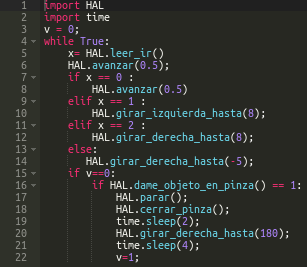
\includegraphics[width=0.65\textwidth, height=0.45\textwidth]{chapters/images/solucionppython.png}
    \caption{Solución en Python}
    \label{fig:my_label}
\end{figure}

\begin{figure}[H]
    \centering
    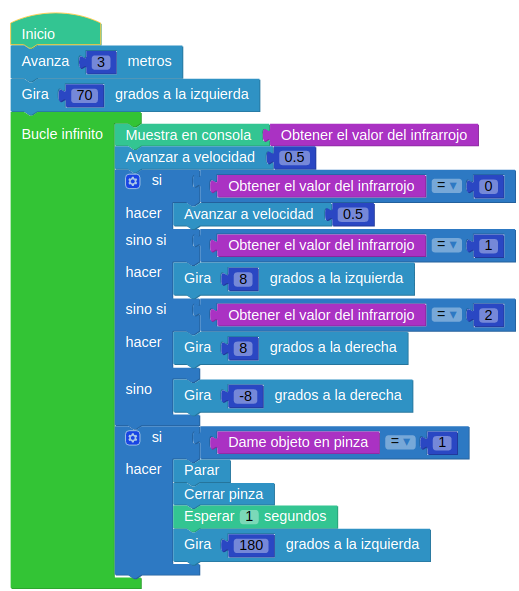
\includegraphics[width=0.65\textwidth, height=0.45\textwidth]{chapters/images/solucionpscratch.png}
    \caption{Solución en Scratch}
    \label{fig:my_label}
\end{figure}